\section{Introduction}
Recurrence relations are central in mathematics and computer science, appearing frequently in problems such as the Fibonacci sequence or divide-and-conquer strategies. While direct computation of recurrence relations can be inefficient, especially for large inputs, transforming them into matrices offers a more efficient alternative.

In this report, we explore how matrix exponentiation can simplify and speed up the computation of recurrence relations. We implement this approach using C++ and compare its performance with a dynamic programming solution, highlighting its advantages for solving high-order or iterative recurrence problems.

\begin{minipage}{\linewidth}
    \centering
    \begin{minipage}{0.32\linewidth}
        \begin{figure}[H]
            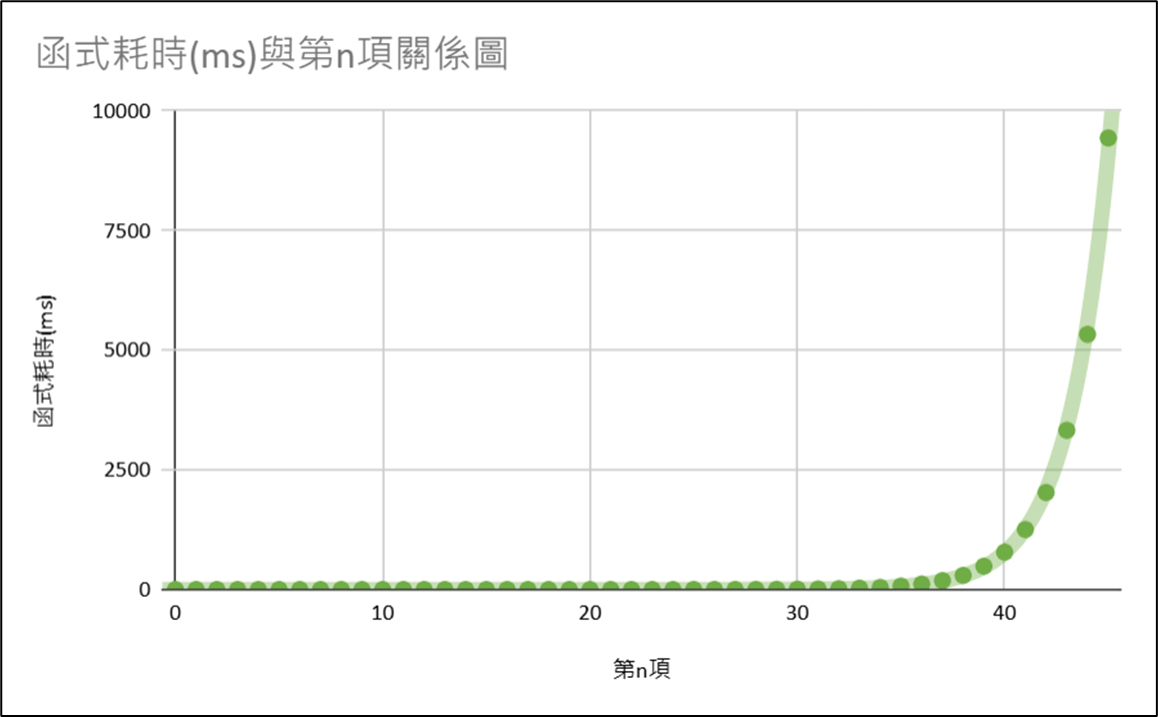
\includegraphics[height=3cm]{picture/fib_re_graph.png}
            \caption{case 1}
            % \label{case1}
        \end{figure}
    \end{minipage}
    % \hspace{0.05\linewidth}
    \begin{minipage}{0.32\linewidth}
        \begin{figure}[H]
            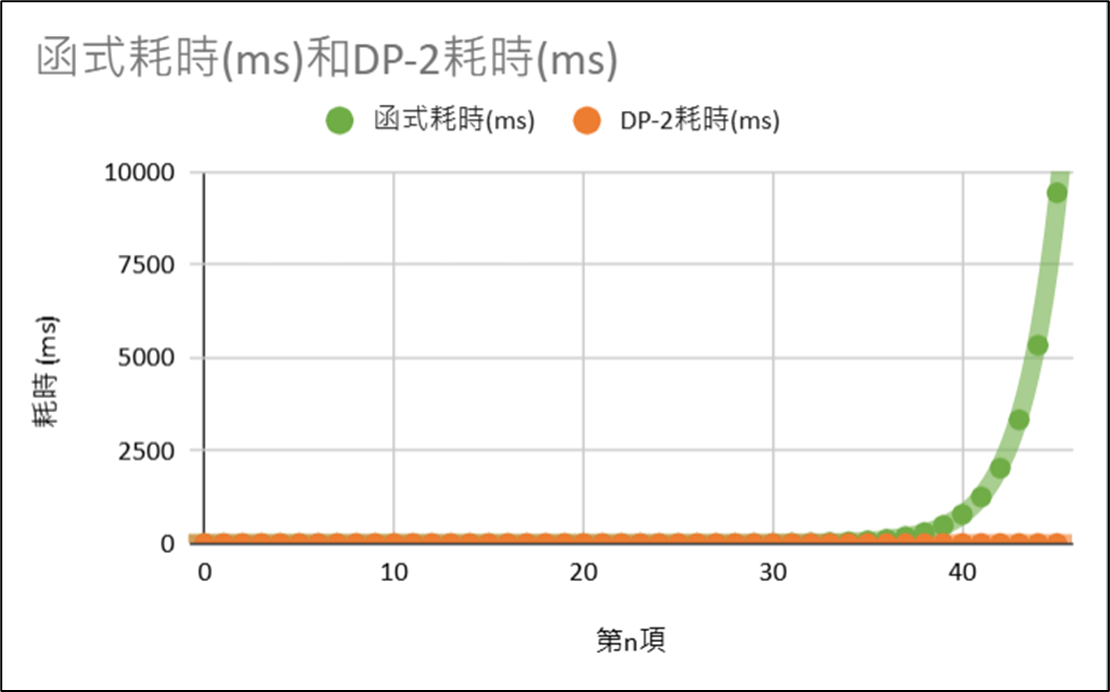
\includegraphics[height=3cm]{picture/fib_re_vs_dp.png}
            \caption{case 2-1}
            % \label{case2-1}
        \end{figure}
    \end{minipage}
    % \hspace{0.05\linewidth}
    \begin{minipage}{0.32\linewidth}
        \begin{figure}[H]
            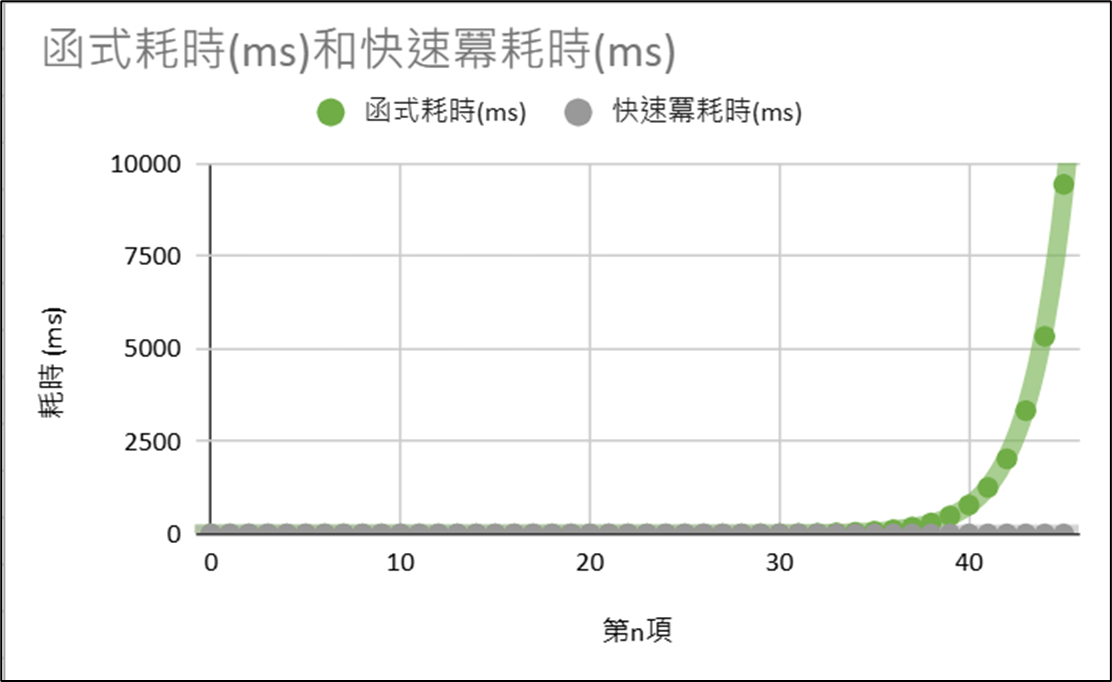
\includegraphics[height=3cm]{picture/fib_re_vs_pow.png}
            \caption{case 2-2}
            % \label{case2-2}
        \end{figure}
    \end{minipage}
\end{minipage}

\section{Materials and Methods}
\subsection{Materials}
Tools and resources utilized include: pen, papers, brains, computers, and the C++ programming language.
\subsection{Methods}
Initially, the transition matrix for the recursive formula is derived, and its theoretical time complexity is calculated. Subsequently, C++ code is implemented to evaluate its performance through execution time measurement. The consistency between the measured execution time and the theoretical time complexity is verified. Finally, the results are compared with those obtained from a dynamic programming (DP) implementation.

\section{Results}

\begin{minipage}{\linewidth}
    \centering
    \begin{minipage}{0.45\linewidth}
        \begin{figure}[H]
            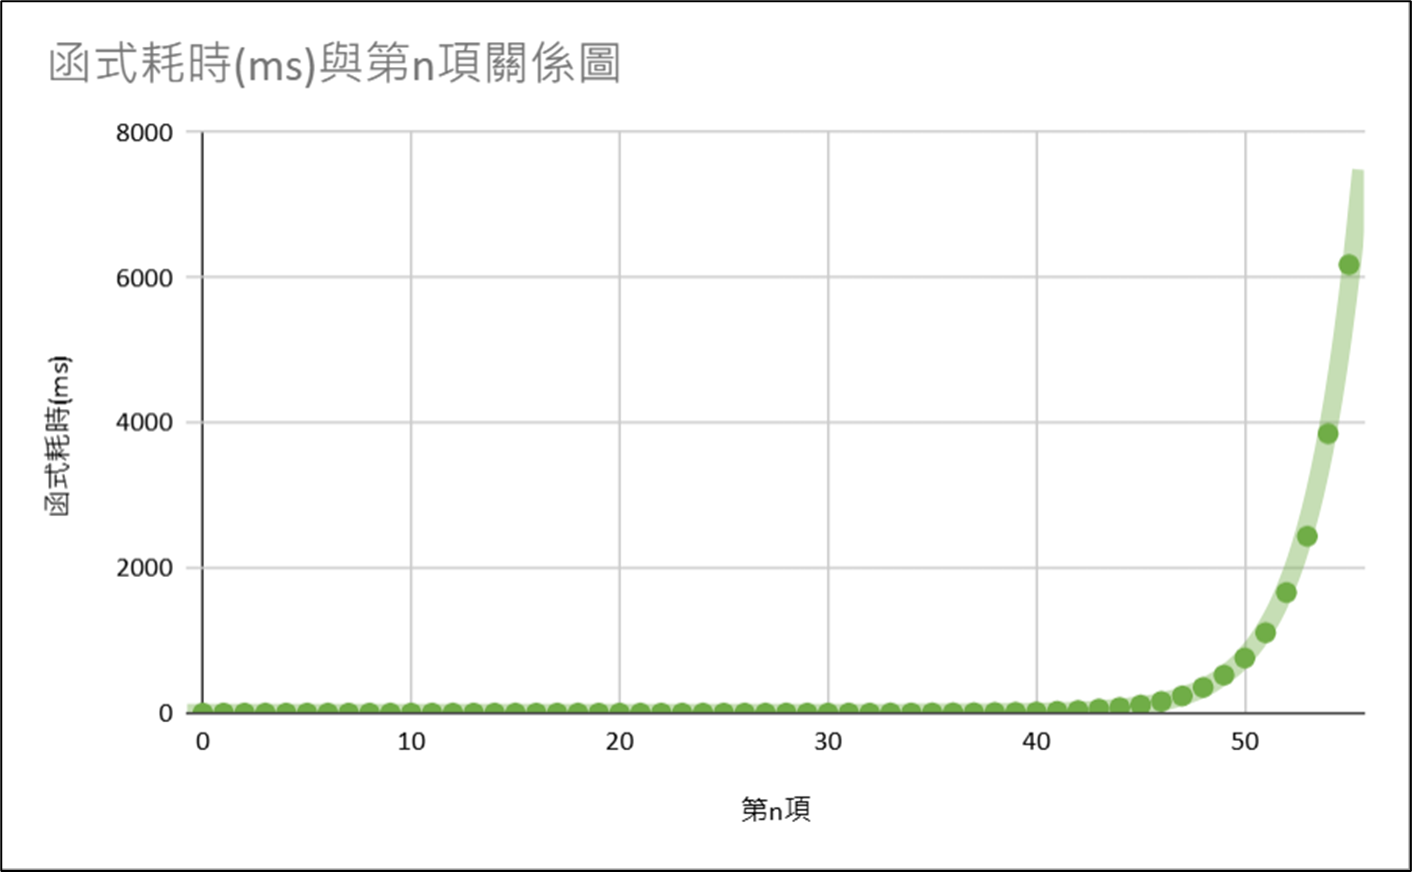
\includegraphics[height=3cm]{picture/rail_re_graph.png}
            \caption{case 1}
            % \label{case1}
        \end{figure}
    \end{minipage}
    % \hspace{0.05\linewidth}
    \begin{minipage}{0.45\linewidth}
        \begin{figure}[H]
            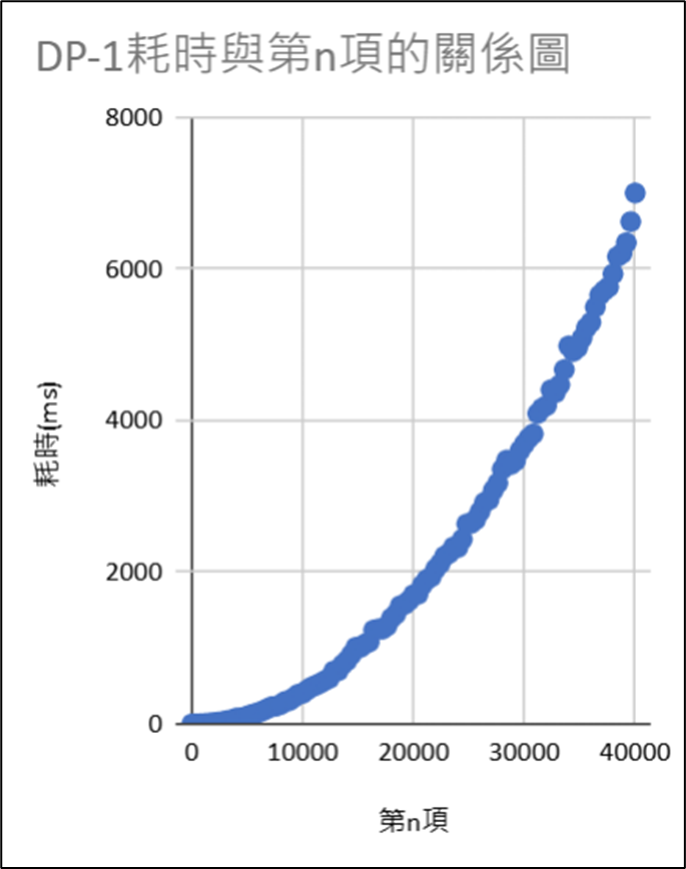
\includegraphics[height=3cm]{picture/rail_dp1.png}
            \caption{case 2-1}
            % \label{case2-1}
        \end{figure}
    \end{minipage}
    \begin{minipage}{0.45\linewidth}
        \begin{figure}[H]
            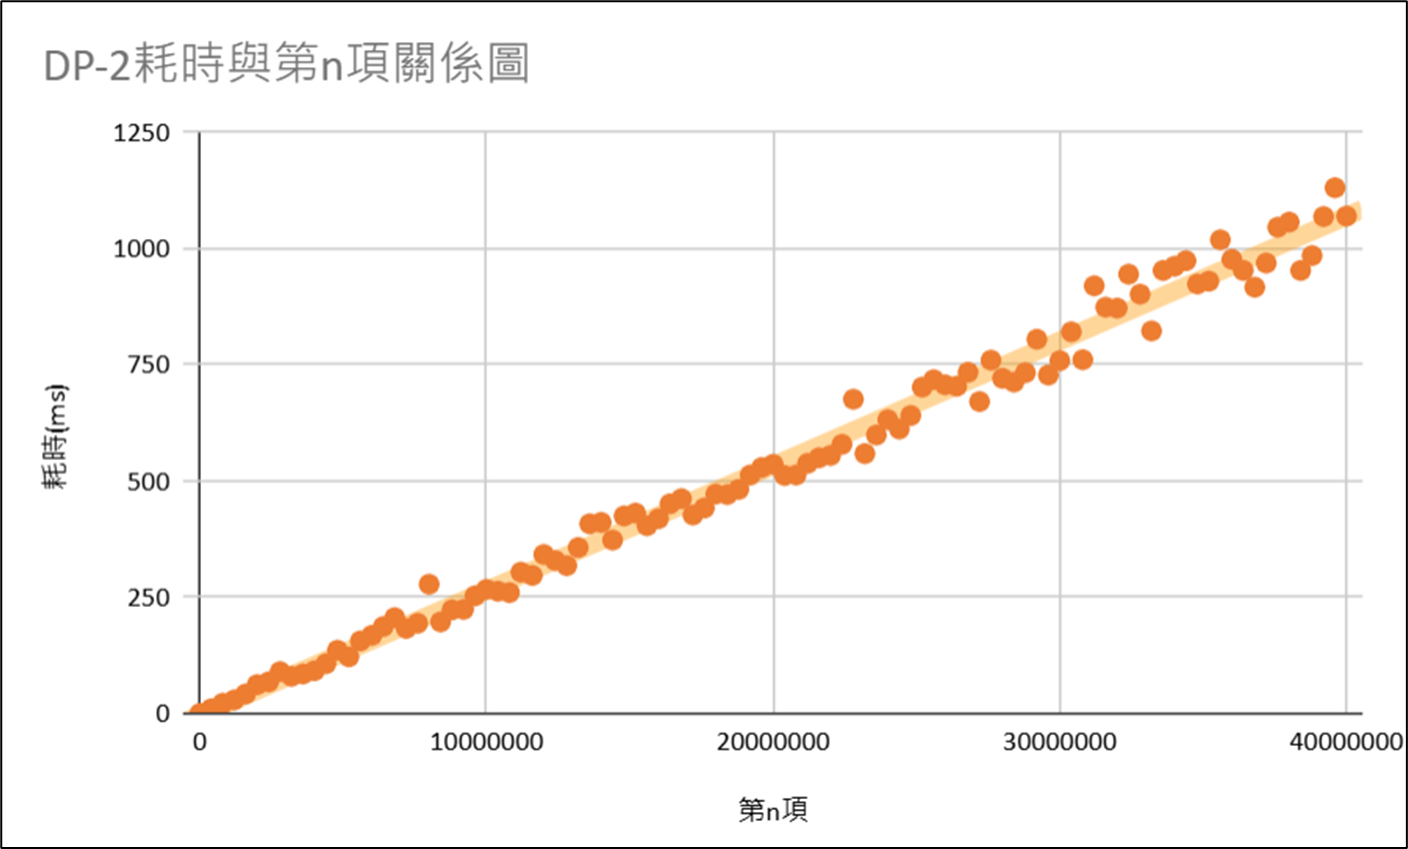
\includegraphics[height=3cm]{picture/rail_dp2.png}
            \caption{case 1}
            % \label{case1}
        \end{figure}
    \end{minipage}
    % \hspace{0.05\linewidth}
    \begin{minipage}{0.45\linewidth}
        \begin{figure}[H]
            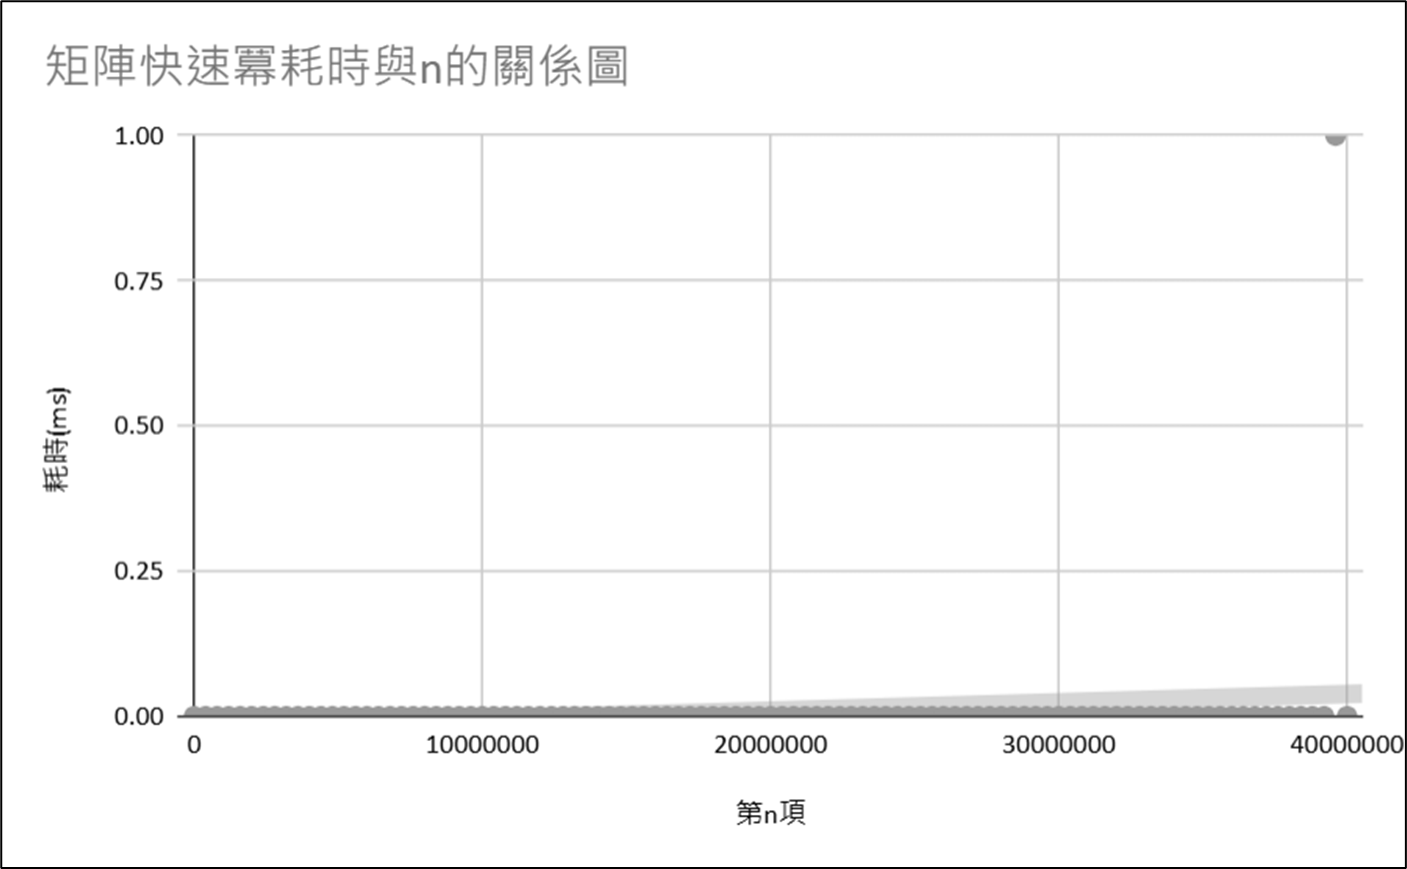
\includegraphics[height=3cm]{picture/rail_pow.png}
            \caption{case 2-1}
            % \label{case2-1}
        \end{figure}
    \end{minipage}
\end{minipage}

\section{Discussion}
\subsection{Fibonacci} 
$F(n) = F(n - 1) + F(n - 2)$

$$ \begin{bmatrix}
        F(n)\\F(n-1)
    \end{bmatrix} =
    \begin{bmatrix}
        1 & 1\\
        1 & 0
    \end{bmatrix}
    \begin{bmatrix}
        F(n - 1)\\
        F(n - 2)
    \end{bmatrix}\\
    = 
    \begin{bmatrix}
        1 & 1\\
        1 & 0
    \end{bmatrix}^{n - 2}
    \begin{bmatrix}
        F(2)\\
        F(1)
    \end{bmatrix}\\
    =
    \begin{bmatrix}
        1 & 1\\
        1 & 0
    \end{bmatrix}^{n - 2}
    \begin{bmatrix}
        1\\
        1
    \end{bmatrix}
$$

\subsection{Rail} $D_i = \sum\limits_{j = 0}^{i - 2}(2(i - j) - 3)D_j$\\

A detailed description of the Rail recurrence relation is provided in Appendix \ref{rail} on page \pageref{rail}.

$$
\begin{bmatrix}
    D_i\\
    D_{i - 1}\\
    D_{i - 2}
\end{bmatrix} = 
\begin{bmatrix}
    2 & 0 & 1\\
    1 & 0 & 0\\
    0 & 1 & 0
\end{bmatrix}
\begin{bmatrix}
    D_{i - 1}\\
    D_{i - 2}\\
    D_{i - 3}
\end{bmatrix} = 
\begin{bmatrix}
    2 & 0 & 1\\
    1 & 0 & 0\\
    0 & 1 & 0
\end{bmatrix}^{i - 2}
\begin{bmatrix}
    D_2\\
    D_1\\
    D_0
\end{bmatrix} = 
\begin{bmatrix}
    2 & 0 & 1\\
    1 & 0 & 0\\
    0 & 1 & 0
\end{bmatrix}^{i - 2}
\begin{bmatrix}
    1\\
    0\\
    1
\end{bmatrix}
$$\\

The complete induction process is detailed in Appendix \ref{induction for Rail} on page \pageref{induction for Rail}.

\section{Conclusion}
\label{conclusion}

\begin{enumerate}
    \item[1.] For recursive relations with fixed coefficients, representing them in matrix form enables efficient computation through repeated multiplication of the same matrix. This approach facilitates the application of fast exponentiation, thereby reducing the number of operations and significantly shortening computation time.\\\
    \item[2.] A comparison between fast exponentiation and the DP approach demonstrates that the time difference becomes increasingly significant as $n$ grows. This observation aligns closely with the theoretical time complexity analysis.
\end{enumerate}

\section{Reference}